\chapter{Cortocircuitos}
No se desarrolla con detalle el tema pues las formulas se encuentran en el formulario, se estudia en otra asignaturas y se prefiere el estudio mediante problemas.
\section{Tipos de cortocircuito}
\begin{figure}[H]
	\centering
	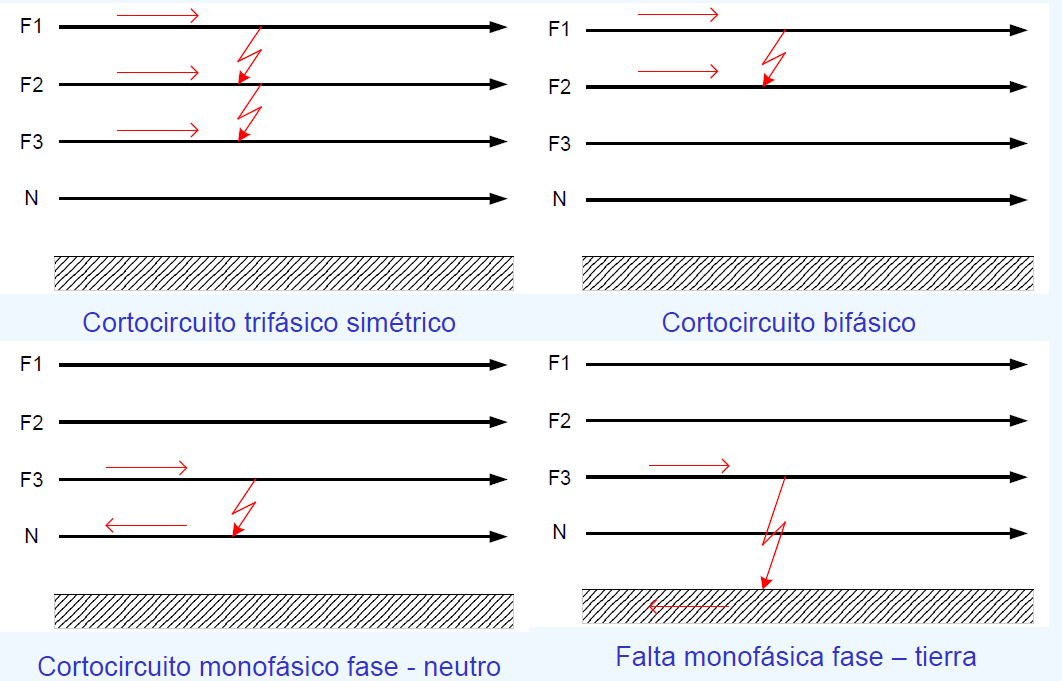
\includegraphics[width=0.7\linewidth]{Images/11}
	\label{fig:11}
\end{figure}
\section{Parámetros de la corriente de cortocircuito}
\begin{itemize}
	\item $I_K^"$: Corriente de cortocircuito simétrica inicial (subtransitoria), valor eficaz
	\begin{itemize}
		\item Corriente de cortocircuito trifásica inicial:$I_{CC}=I_{K}^"$
		\item Corriente de cortocircuito bifásica inicial: $I_{CC2F}=I_{K2}^"$
		\item Corriente de cortocircuito monofásica inicial: $I_{CC1F}=I_{K1}^"$
	\end{itemize}
	\item $i_p$: Valor de cresta de la corriente de cortocircuito, $i_p\approx 2.5 I_K^"$
	\item $A$: Valor inicial de la corriente continua
	\item $I_K$: Corriente de cortocircuito permanente
\end{itemize}
\section{Validez de cálculo}
Se realiza el cálculo bajo la norma UNE EN 60909:2001 Cálculo de corrientes de cortocircuito en sistemas trifásicos de corriente alterna. Tiene validez para cortocircuitos monofásicos, bifásicos y trifásicos con neutro rígido o impedante. No es válido para cortocircuitos monofásicos con bobina Petersen (resonante) o neutro aislante.
\section{Factor de tensión}
Para tener en cuenta la variabilidad de la tensión del sistema se toma un valor del $\pm5\%$ para baja tensión y un $+10\%$ en alta tensión. Esto significa que en baja tensión el parámetro c esta comprendido entre 0,95 y 1,05 mientras que en alta tensión el parámetro c esta comprendido entre 1 y 1,1.
\section{Hipótesis del cálculo}
\begin{itemize}
	\item No hay cambio en el tipo de cortocircuito mientras dura éste
	\item No hay cambio de la red involucrada
	\item La impedancia de los transformadores es la correspondiente a la toma principal de los cambiadores de tomas
	\item No se tienen en cuenta las resistencias de arco
	\item Se desprecian todas las capacidades de línea, admitancias en derivación y cargas no rotativas, excepto las del sistema homopolar
\end{itemize}
\section{Condiciones de corriente de cortocircuito máxima}
\begin{itemize}
	\item Factor de tensión “c” máximo
	\item Configuración del sistema que de lugar a la corriente de cortocircuito máxima
	\item Máxima contribución de las redes de alimentación: Impedancia de redes externas mínima
	\item Impedancia de cables y líneas a 20$^\circ$C
	\item Debe incluirse, en su caso, la aportación de motores
	\item En el cuadro principal el cortocircuito puede ser monofásico o trifásico mientras que en los cuadros secundarios normalmente es monofásico
\end{itemize}
\section{Condiciones de corriente de cortocircuito mínima}
\begin{itemize}
	\item Factor de tensión “c” mínimo
	\item Configuración del sistema que de lugar a la corriente de cortocircuito mínima
	\item Mínima contribución de las redes de alimentación
	\item Impedancia de cables y líneas a la temperatura al final de la duración del cortocircuito. Normalmente a 150$^\circ$C
	\item No se considera la aportación de motores
	\item Puede ser la corriente monofásica o bifásica
\end{itemize}
\section{Aportación de motores}
La contribución de motores asíncronos en sistemas de potencia de BT a la corriente de cortocircuito se puede despreciarsi se cumple que la suma de corrientes nominales de los motores es menor al 1\% de la corriente de cortocircuito simétrica inicial.
\newline

No se debe considerar la aportación de aquellos motores que por su control o proceso no estén conectados cuando se da el cortocircuito. 
\newline

Se puede despreciar la corriente de descarga de los condensadores en el cálculo del valor de cresta de la corriente de cortocircuito.
\newline

Se considera la contribución del motor como 8 veces su intensidad nominal y si esta alimentado por un convertidor estático reversible como 3 veces su intensidad nominal. 
\newline

Se considera la aportación de los motores al cuadro principal siempre, pero si están en ramas diferentes del esquema unifilar se considera que un motor no aporta, es decir, si los motores están en diferentes cuadros secundarios no aportan corriente al cortocircuito (están demasiado alejados como para ver el 0 de tensión).
\section{Métodos de cálculo simplificados}
Son métodos que se pueden utilizar cuando no se conocen los valores de R y X de la instalación. Suele ser suficientemente exacto hasta los 800kVA y se basa en asumir el mismo factor de potencia desde el origen del circuito hasta el defecto.
\newline

Se sustituye la impedancia de la alimentación por una caída de tensión y considera sólo la parte resistiva de la impedancia de los cables. Es válido para cortocircuitos monofásicos en circuitos terminales (lejos del centro de transformación).
\newline

Las hipótesis de cálculo son:
\begin{itemize}
	\item Defecto fase -neutro como más desfavorable
	\item La tensión en el momento del defecto vale el 80 \% de la nominal en el origen del circuito
	\item Se consideran despreciables las inductancias de los cables
	\item El cálculo de las resistencias de los conductores a 20$^\circ$C
\end{itemize}